\chapter{AttOmics supplementary}\label{chap:attomics_appendix}
\begin{table}[htbp]
	\centering
	\caption{Distribution of the samples across cancer and splits}\label{tab:cancer_rep}
	\begin{tblr}{
		colspec={
				Q[l,m]
				Q[si={table-format=3,table-number-alignment=center},r]
				Q[si={table-format=3,table-number-alignment=center},r]
				Q[si={table-format=3,table-number-alignment=center},r]
				Q[si={table-format=3,table-number-alignment=center},r]
			},%
		row{1} = {guard, c, font=\bfseries},%
		row{2-Z} = {font=\small},%
		hline{1,Z} = {2pt},%
		hline{2,Y} = {1pt},%
				cell{Z}{1}={font=\bfseries},%
			}
		Cancer & Train & Validation & Test & Total \\
		BRCA   & 740   & 159        & 159  & 1058  \\
		UCEC   & 368   & 79         & 80   & 527   \\
		LGG    & 366   & 79         & 79   & 524   \\
		KIRC   & 355   & 76         & 77   & 508   \\
		THCA   & 354   & 76         & 76   & 506   \\
		LUAD   & 353   & 76         & 76   & 505   \\
		HNSC   & 344   & 74         & 74   & 492   \\
		PRAD   & 342   & 73         & 74   & 489   \\
		LUSC   & 331   & 71         & 71   & 473   \\
		SKCM   & 313   & 67         & 68   & 448   \\
		COAD   & 303   & 65         & 66   & 434   \\
		BLCA   & 282   & 60         & 61   & 403   \\
		OV     & 261   & 56         & 57   & 374   \\
		STAD   & 259   & 55         & 56   & 370   \\
		LIHC   & 257   & 55         & 56   & 368   \\
		Normal & 252   & 54         & 55   & 361   \\
		CESC   & 205   & 44         & 44   & 293   \\
		KIRP   & 200   & 43         & 44   & 287   \\
		SARC   & 182   & 39         & 39   & 260   \\
		LAML   & 67    & 15         & 15   & 97    \\
		Total  & 6134  & 1316       & 1327 & 8777
	\end{tblr}
\end{table}

\begin{table}[htbp]
	\centering
	\caption{Graph dimension for the GCN model}\label{tab:graph_dim}
	\begin{tblr}{
		colspec={
				Q[l,m]
				Q[l,m]
				Q[si={table-format=3,table-number-alignment=center},r]
				Q[si={table-format=3,table-number-alignment=center},r]
			},%
		row{1} = {guard, c, font=\bfseries},%
		row{2-Z} = {font=\small},%
		hline{1,Z} = {2pt},%
				hline{2} = {1pt},%
				hline{3} = {dashed, 1pt},
				cell{3}{1} = {r=3,c=1}{m},
			}
		Graph & Omics & Nodes & Edges  \\
		PPI   & mRNA  & 15985 & 234984 \\
		CoExp & mRNA  & 17951 & 400632 \\
		      & miRNA & 314   & 1051   \\
		      & DNAm  & 8360  & 390455
	\end{tblr}
\end{table}

\begin{table}[htbp]
	\centering
	\caption{Tested values of the hyper-parameters for the different architectures.}\label{tab:search_space}
	\begin{tblr}{
		colspec={
				Q[l,m]
				Q[l,m]
				Q[r,m]
			},%
		row{1} = {font=\bfseries},%
		row{2-Z} = {font=\small},%
		hline{1,Z} = {2pt},%
		hline{2} = {1pt},%
		hline{6,9,12,15,21} = {dashed, 1pt},%
				cell{2}{1} = {r=4,c=1}{l,m},%
				cell{6}{1} = {r=3,c=1}{l,m},%
				cell{9}{1} = {r=3,c=1}{l,m},%
				cell{12}{1} = {r=3,c=1}{l,m},%
				cell{15}{1} = {r=6,c=1}{l,m},%
				cell{21}{1} = {r=6,c=1}{l,m},%
			}
		Model         & Hyper-parameter     & Tested values                 \\
		MLP           & Nb layers           & \([ |1, 20 |]\)               \\
		              & Reduction ratio     & \([0.1, 0.9]\)                \\
		              & Dropout             & \([0,1]\)                     \\
		              & Batch norm.         & True/False                    \\
		CNN1d         & Kernel size         & 2,4,8                         \\
		              & Pooling size        & 2,4                           \\
		              & Num channels        & 32, 64, 128                   \\
		GNN           & Kernel size         & X, 2, 4, 8                    \\
		              & Num channels        & 1, 16, 32                     \\
		              & Readout             & concatenate, max, mean        \\
		SVM           & C                   & 0.1, 1, 10, 100, 1000         \\
		              & gamma               & 1, 0.1, 0.01, 0.001, 0.0001   \\
		              & Kernel              & rbf, linear, poly, sigmoid    \\
		Random Forest & n\_estimators       & \([1, 100]\)                  \\
		              & max\_features       & auto, sqrt                    \\
		              & max\_depth          & \([3, 20]\)                   \\
		              & min\_sample\_splits & 2, 5, 10, 15, 20, 25, 30, 50  \\
		              & min\_samples\_leaf  & 1, 2, 4, 6, 8, 10, 20, 30, 50 \\
		              & bootstrap           & True/False                    \\
		XGBoost       & n\_estimators       & \([1, 100]\)                  \\
		              & max\_depth          & 3, 4, 5, 6, 8, 10, 12, 15     \\
		              & gamma               & 0.0, 0.1, 0.2, 0.3, 0.4       \\
		              & min\_child\_weight  & 1, 3, 5, 7                    \\
		              & colsample\_bytree   & 0.3, 0.4, 0.5, 0.7            \\
		              & learning\_rate      & 0.05,0.10,0.15,0.20,0.25,0.30
	\end{tblr}
\end{table}

\begin{table}[htbp]
	\centering
	\caption{Selected hyper-parameters for the AttOmics architecture.}\label{tab:attomics_hparams}
	\begin{tblr}{
		colspec={
				Q[l,m]
				Q[l,m]
				Q[r,m]
				Q[r,m]
				Q[r,m]
			},%
		row{1} = {font=\bfseries},%
		row{2-Z} = {font=\small},%
		hline{1,Z} = {2pt},%
		hline{2} = {1pt},%
		hline{6,10} = {dashed, 1pt},%
				cell{2}{1} = {r=4,c=1}{l,m},%
				cell{6}{1} = {r=4,c=1}{l,m},%
				cell{10}{1} = {r=4,c=1}{l,m},%
			}
		Grouping   & Parameter  & mRNA                & DNAm           & miRNA   \\
		Random     & \# group   & 20                  & 10             & 5       \\
		           & \# blocks  & 4                   & 3              & 2       \\
		           & \# heads   & 1                   & 1              & 1       \\
		           & group size & 2164, 1459, 754, 50 & 1552, 826, 100 & 201, 80 \\
		Clustering & \# group   & 20                  & 20             & 10      \\
		           & \# blocks  & 4                   & 3              & 1       \\
		           & \# heads   & 1                   & 1              & 1       \\
		           & group size & 2164, 1459, 754, 50 & 776, 413, 50   & 50      \\
		GO         & \# group   & 46                  &                &         \\
		           & \# blocks  & 3                   &                &         \\
		           & \# heads   & 1                   &                &         \\
		           & group size & 200, 105, 10        &                &
	\end{tblr}
\end{table}

\begin{table}[htbp]
	\centering
	\caption{Architecture used for the models. X not applicable. For the GCN model a - kernel means convolution from spatial space, and \(>0\) means convolution in the spectral space}\label{tab:arch_other}% chktex 8
	\begin{tblr}{
		colspec={
				Q[l,m]
				Q[l,m]
				Q[r,m]
				Q[r,m]
				Q[r,m]
			},%
		row{1} = {font=\bfseries},%
		row{2-Z} = {font=\small},%
		hline{1,Z} = {2pt},%
		hline{2} = {1pt},%
		hline{5,9,12,15,18,24} = {dashed, 1pt},%
				cell{2}{1} = {r=3,c=1}{l,m},%
				cell{5}{1} = {r=4,c=1}{l,m},%
				cell{9}{1} = {r=3,c=1}{l,m},%
				cell{12}{1} = {r=3,c=1}{l,m},%
				cell{15}{1} = {r=3,c=1}{l,m},%
				cell{18}{1} = {r=6,c=1}{l,m},%
				cell{24}{1} = {r=6,c=1}{l,m},%
			}
		Model         & Parameter          & mRNA      & DNAm        & miRNA    \\
		MLP           & hidden dim         & 5739, 646 & 13675, 4103 & 807, 485 \\
		              & dropout            & 0         & 0           & 0        \\
		              & batch norm         & True      & True        & True     \\
		CNN --- 1D    & kernel             & 4         & 2           & 2        \\
		              & pooling            & 4         & 2           & 2        \\
		              & \# channels        & 64        & 64          & 64       \\
		              & stride             & 1         & 1           & 1        \\
		GNN --- PPI   & \# channels        & 1         & X           & X        \\
		              & kernel             & 2         & X           & X        \\
		              & readout            & concat    & X           & X        \\
		GNN --- CoExp & \# channels        & 1         & 1           & 1        \\
		              & kernel             & -         & -           & 2        \\ % chktex 8
		              & readout            & concat    & concat      & concat   \\
		SVM           & kernel             & rbf       & rbf         & linear   \\
		              & gamma              & 0.0001    & 0.0001      & 1        \\
		              & C                  & 100       & 1000        & 0.1      \\
		RF            & n\_estimators      & 95        & 88          & 99       \\
		              & min\_samples       & 10        & 2           & 5        \\
		              & min\_samples\_leaf & 1         & 1           & 1        \\
		              & max\_features      & sqrt      & auto        & sqrt     \\
		              & max\_depth         & 18        & None        & 16       \\
		              & bootstrap          & False     & False       & False    \\
		XGBoost       & n\_estimators      & 88        & 18          & 66       \\
		              & min\_child\_weight & 7         & 7           & 7        \\
		              & max\_depth         & 15        & 4           & 15       \\
		              & learning\_rate     & 0.15      & 0.25        & 0.15     \\
		              & gamma              & 0         & 0.2         & 0.4      \\
		              & colsample\_bytree  & 0.5       & 0.5         & 0.5
	\end{tblr}
\end{table}

\begin{table}[htbp]
	\sisetup{separate-uncertainty-units=single, separate-uncertainty,detect-mode}
	\centering
	\caption{Models' sizes and their associated performances.}\label{tab:n_params_arch}
	\begin{tblr}{
		colspec={
				Q[l,m]
				Q[l,m]
				Q[r,m]
				Q[si={table-format=1.3(3),table-number-alignment=center, table-align-uncertainty = true}]
				Q[si={table-format=1.3(3),table-number-alignment=center, table-align-uncertainty = true}]
			},%
		row{1} = {guard, c},%
		row{2-Z} = {font=\small},%
		hline{1,Z} = {2pt},%
		hline{2} = {1pt},%
		hline{10,21} = {1pt, dashed},
				cell{2}{1} = {r=8,c=1}{l,m},
				cell{10}{1} = {r=11,c=1}{l,m},
				cell{21}{1} = {r=8,c=1}{l,m},
			}
		Omics & Model                   & \# of parameters & Error-Rate & C-Index   \\
		DNAm  & AttOmics --- Clustering & 28M              & 0.034(2)   & 0.722(10) \\
		      & AttOmics --- Random     & 62M              & 0.034(1)   & 0.721(5)  \\
		      & CNN1d                   & 93M              & 0.042(1)   & 0.720(8)  \\
		      & MLP                     & 367M             & 0.039(2)   & 0.718(2)  \\
		      & GNN --- CoExp           & 8.6M             & 0.037(3)   & 0.708(4)  \\
		      & SVM                     &                  & 0.034(0)   &           \\
		      & RF                      &                  & 0.050(3)   &           \\
		      & XGBoost                 &                  & 0.051(0)   &           \\
		mRNA  & AttOmics --- Clustering & 240M             & 0.043(2)   & 0.723(6)  \\
		      & AttOmics --- GO         & 28M              & 0.040(2)   & 0.721(5)  \\
		      & AttOmics --- Hallmarks  & 1.9M             & 0.046(3)   & 0.722(9)  \\
		      & AttOmics --- Random     & 240M             & 0.040(2)   & 0.726(6)  \\
		      & CNN1d                   & 470M             & 0.054(1)   & 0.714(6)  \\
		      & MLP                     & 333M             & 0.047(2)   & 0.717(6)  \\
		      & GNN --- CoExp           & 19M              & 0.047(2)   & 0.718(12) \\
		      & GNN --- PPI             & 16M              & 0.047(1)   & 0.722(3)  \\
		      & SVM                     &                  & 0.054(0)   &           \\
		      & RF                      &                  & 0.058(1)   &           \\
		      & XGBoost                 &                  & 0.035(0)   &           \\
		miRNA & AttOmics --- Clustering & 0.22M            & 0.071(4)   & 0.679(9)  \\
		      & AttOmics --- Random     & 0.68M            & 0.077(3)   & 0.668(2)  \\
		      & CNN1d                   & 6.6M             & 0.120(5)   & 0.677(4)  \\
		      & MLP                     & 1.7M             & 0.077(7)   & 0.669(11) \\
		      & GNN --- CoExp           & 0.37M            & 0.082(12)  & 0.697(13) \\
		      & SVM                     &                  & 0.034(0)   &           \\
		      & RF                      &                  & 0.050(3)   &           \\
		      & XGBoost                 &                  & 0.051(0)   &           \\
	\end{tblr}
\end{table}



\begin{table}[htbp]
	\sisetup{detect-mode}
	\centering
	\caption{Classification performances of the different models}\label{tab:perf_results}
	% TODO: longtblr
	\begin{tblr}{
		colspec={
				Q[l,m, colsep=2pt]
				Q[l,m, colsep=2pt]
				Q[si={table-format=1.3(3),table-number-alignment=center, table-align-uncertainty = true}, colsep=2pt]
				Q[si={table-format=1.3(3),table-number-alignment=center, table-align-uncertainty = true}, colsep=2pt]
				Q[si={table-format=1.3(3),table-number-alignment=center, table-align-uncertainty = true}, colsep=2pt]
				Q[si={table-format=1.3(3),table-number-alignment=center, table-align-uncertainty = true}, colsep=2pt]
				Q[si={table-format=1.3(3),table-number-alignment=center, table-align-uncertainty = true}, colsep=2pt]
				Q[si={table-format=1.3(3),table-number-alignment=center, table-align-uncertainty = true}, colsep=2pt]
			},%
		row{1} = {guard},%
		row{2-Z} = {font=\footnotesize},%
		hline{1,Z} = {2pt},%
		hline{2} = {1pt},%
		hline{10,21} = {1pt, dashed},
				cell{2}{1} = {r=8,c=1}{l,m},
				cell{10}{1} = {r=11,c=1}{l,m},
				cell{21}{1} = {r=8,c=1}{l,m},
			}
		Omics & Model                   & AUROC    & Accuracy  & F1-Score  & Precision & Recall    & Specificity \\
		DNAm  & AttOmics --- Clustering & 0.999(0) & 0.966(02) & 0.965(02) & 0.965(02) & 0.966(02) & 0.998(0)    \\
		      & AttOmics --- Random     & 0.999(0) & 0.966(01) & 0.964(02) & 0.963(02) & 0.966(01) & 0.998(0)    \\
		      & CNN1d                   & 0.998(0) & 0.958(01) & 0.956(01) & 0.955(01) & 0.958(01) & 0.998(0)    \\
		      & GCN --- CoExp           & 0.999(0) & 0.963(03) & 0.962(04) & 0.961(05) & 0.963(03) & 0.998(0)    \\
		      & MLP                     & 0.999(0) & 0.961(02) & 0.961(02) & 0.961(02) & 0.961(02) & 0.998(0)    \\
		      & RF                      & 0.998(0) & 0.950(03) & 0.950(03) & 0.950(03) & 0.950(03) & 0.997(0)    \\
		      & SVM                     & 0.998(0) & 0.966(00) & 0.966(00) & 0.966(00) & 0.966(00) & 0.998(0)    \\
		      & XGBoost                 & 0.997(0) & 0.949(00) & 0.949(00) & 0.949(00) & 0.949(00) & 0.997(0)    \\
		mRNA  & AttOmics --- Clustering & 0.999(0) & 0.957(02) & 0.956(02) & 0.956(02) & 0.957(02) & 0.998(0)    \\
		      & AttOmics --- GO         & 0.999(0) & 0.960(02) & 0.960(02) & 0.960(02) & 0.960(02) & 0.998(0)    \\
		      & AttOmics --- Hallmarks  & 0.999(0) & 0.954(03) & 0.954(04) & 0.953(04) & 0.954(03) & 0.998(0)    \\
		      & AttOmics --- Random     & 0.998(0) & 0.960(02) & 0.960(02) & 0.960(02) & 0.960(02) & 0.998(0)    \\
		      & CNN1d                   & 0.997(0) & 0.946(03) & 0.946(03) & 0.947(03) & 0.946(03) & 0.997(0)    \\
		      & GCN --- CoExp           & 0.999(0) & 0.953(02) & 0.953(02) & 0.954(02) & 0.953(02) & 0.998(0)    \\
		      & GCN --- PPI             & 0.999(0) & 0.953(01) & 0.953(01) & 0.954(02) & 0.953(01) & 0.998(0)    \\
		      & MLP                     & 0.997(0) & 0.953(02) & 0.954(02) & 0.955(02) & 0.953(02) & 0.998(0)    \\
		      & RF                      & 0.998(0) & 0.942(01) & 0.942(01) & 0.942(01) & 0.942(01) & 0.997(0)    \\
		      & SVM                     & 0.997(0) & 0.946(00) & 0.946(00) & 0.946(00) & 0.946(00) & 0.997(0)    \\
		      & XGBoost                 & 0.999(0) & 0.965(00) & 0.965(00) & 0.965(00) & 0.965(00) & 0.998(0)    \\
		miRNA & AttOmics --- Clustering & 0.997(0) & 0.929(04) & 0.927(04) & 0.927(05) & 0.929(04) & 0.996(0)    \\
		      & AttOmics --- Random     & 0.996(0) & 0.923(03) & 0.922(03) & 0.923(03) & 0.923(03) & 0.996(0)    \\
		      & CNN1d                   & 0.990(0) & 0.880(05) & 0.875(05) & 0.875(06) & 0.880(05) & 0.994(0)    \\
		      & GCN --- CoExp           & 0.995(1) & 0.918(12) & 0.915(13) & 0.914(13) & 0.918(12) & 0.996(1)    \\
		      & MLP                     & 0.995(0) & 0.923(07) & 0.923(07) & 0.924(08) & 0.923(07) & 0.996(0)    \\
		      & RF                      & 0.997(0) & 0.941(02) & 0.941(02) & 0.941(02) & 0.941(02) & 0.997(0)    \\
		      & SVM                     & 0.994(0) & 0.924(00) & 0.924(00) & 0.924(00) & 0.924(00) & 0.996(0)    \\
		      & XGBoost                 & 0.998(0) & 0.956(00) & 0.956(00) & 0.956(00) & 0.956(00) & 0.998(0)
	\end{tblr}
\end{table}

\begin{landscape}
	\begin{table}
		\tiny
		\centering
		\caption{P-value from the t-test on the error rate of the different models}\label{tab:pval_error_rate}
		\begin{tabular}{llrrrrrrrrrr}
			\toprule
			omics                  & Model                   & AttOmics --- GO & AttOmics --- Hallmarks & AttOmics --- Random & CNN1d & GCN --- CoExp & MLP      & RF    & SVM      & XGBoost  & GCN --- PPI \\
			\midrule
			\multirow{7}{*}{DNAm}  & AttOmics --- Clustering & -               & -                      & 1.00                & 0.083 & 0.083         & 0.083    & 0.083 & 0.648    & 0.083    & -           \\ % chktex 8
			                       & AttOmics --- Random     & -               & -                      & -                   & 0.083 & 0.381         & 0.083    & 0.083 & 0.648    & 0.083    & -           \\ % chktex 8
			                       & CNN1d                   & -               & -                      & -                   & -     & 0.083         & 0.083    & 0.083 & 0.083    & 0.083    & -           \\ % chktex 8
			                       & GCN --- CoExp           & -               & -                      & -                   & -     & -             & 0.510417 & 0.083 & 0.159091 & 0.083    & -           \\ % chktex 8
			                       & MLP                     & -               & -                      & -                   & -     & -             & -        & 0.083 & 0.083    & 0.083    & -           \\ % chktex 8
			                       & RF                      & -               & -                      & -                   & -     & -             & -        & -     & 0.083    & 0.648148 & -           \\ % chktex 8
			                       & SVM                     & -               & -                      & -                   & -     & -             & -        & -     & -        & 0.083    & -           \\ % chktex 8
			\midrule
			\multirow{10}{*}{mRNA} & AttOmics --- Clustering & 0.219           & 0.149                  & 0.078               & 0.078 & 0.078         & 0.078    & 0.078 & 0.078    & 0.078    & 0.078       \\
			                       & AttOmics --- GO         & -               & 0.149                  & 0.828               & 0.078 & 0.078         & 0.078    & 0.078 & 0.078    & 0.078    & 0.078       \\ % chktex 8
			                       & AttOmics --- Hallmarks  & -               & -                      & 0.078               & 0.078 & 0.661         & 0.661    & 0.078 & 0.078    & 0.078    & 0.661       \\ % chktex 8
			                       & AttOmics --- Random     & -               & -                      & -                   & 0.078 & 0.078         & 0.078    & 0.078 & 0.078    & 0.078    & 0.078       \\ % chktex 8
			                       & CNN1d                   & -               & -                      & -                   & -     & 0.078         & 0.078    & 0.078 & 0.828    & 0.078    & 0.078       \\ % chktex 8
			                       & GCN --- CoExp           & -               & -                      & -                   & -     & -             & 0.501    & 0.078 & 0.078    & 0.078    & 0.661       \\ % chktex 8
			                       & GCN --- PPI             & -               & -                      & -                   & -     & -             & 1.00     & 0.078 & 0.078    & 0.078    & -           \\ % chktex 8
			                       & MLP                     & -               & -                      & -                   & -     & -             & -        & 0.078 & 0.078    & 0.078    & -           \\ % chktex 8
			                       & RF                      & -               & -                      & -                   & -     & -             & -        & -     & 0.078    & 0.078    & -           \\ % chktex 8
			                       & SVM                     & -               & -                      & -                   & -     & -             & -        & -     & -        & 0.078    & -           \\ % chktex 8
			\midrule
			\multirow{7}{*}{miRNA} & AttOmics --- Clustering & -               & -                      & 0.159               & 0.092 & 0.159         & 0.159    & 0.092 & 0.092    & 0.092    & -           \\ % chktex 8
			                       & AttOmics --- Random     & -               & -                      & -                   & 0.092 & 0.510         & 1.00     & 0.092 & 0.673    & 0.092    & -           \\ % chktex 8
			                       & CNN1d                   & -               & -                      & -                   & -     & 0.092         & 0.092    & 0.092 & 0.092    & 0.092    & -           \\ % chktex 8
			                       & GCN --- CoExp           & -               & -                      & -                   & -     & -             & 0.673    & 0.092 & 0.510    & 0.092    & -           \\ % chktex 8
			                       & MLP                     & -               & -                      & -                   & -     & -             & -        & 0.092 & 1.00     & 0.092    & -           \\ % chktex 8
			                       & RF                      & -               & -                      & -                   & -     & -             & -        & -     & 0.092    & 0.092    & -           \\ % chktex 8
			                       & SVM                     & -               & -                      & -                   & -     & -             & -        & -     & -        & 0.092    & -           \\ % chktex 8
			\bottomrule
		\end{tabular}
	\end{table}
\end{landscape}


\begin{figure}[htbp]
	\centering
	\begin{tikzpicture}
		\begin{groupplot}[group style={
						group size=2 by 2,
						horizontal sep=__ATTOMICSHSEP__,
						vertical sep=__ATTOMICSVSEP__,
						xlabels at=edge bottom,
						ylabels at=edge left,
						xticklabels at=all,
						yticklabels at=all,
						group name=perfattomics
					},
				tick label style={/pgf/number format/assume math mode=true},
				xtick=data, xlabel=Number of training examples, ylabel=Test Precision, minor y tick num=5,legend cell align={left}, legend style={draw=none},xtick pos=bottom, ytick pos = left, scaled y ticks=false,
				yticklabel style={
						/pgf/number format/fixed,
						/pgf/number format/precision=2
					}, height=__ATTOMICSHEIGHT__, width=__ATTOMICSWIDTH__, title style={yshift=-1.2ex, font=\small}
			]
			\nextgroupplot[title=\textbf{DNAm}]
			\attomicsplotomics{y__DNAm__}{\attomicsperfprecision}
			\draw[gray] (axis cs:5900,0.945) rectangle (axis cs:6368,0.968);
			\coordinate (dnamx1) at (axis cs:5900,0.945);
			\coordinate (dnamx2) at (axis cs:6368,0.945);
			\nextgroupplot[legend to name={attomicsprecisionleg}, legend style={legend columns=1}, title=\textbf{mRNA}]
			\attomicsplotomics{y__mRNA__}{\attomicsperfprecision}
			\draw[gray] (axis cs:5900,0.937) rectangle (axis cs:6368,0.968);
			\coordinate (mrnax1) at (axis cs:5900,0.937);
			\coordinate (mrnax2) at (axis cs:6368,0.937);
			\nextgroupplot[title=\textbf{miRNA}]
			\attomicsplotomics{y__miRNA__}{\attomicsperfprecision}
			\draw[gray] (axis cs:5900,0.865) rectangle (axis cs:6368,0.965);
			\coordinate (mirnax1) at (axis cs:5900,0.865);
			\coordinate (mirnax2) at (axis cs:6368,0.865);
			\nextgroupplot[group/empty plot]
		\end{groupplot}

		\node at (perfattomics c1r2.east -| perfattomics c2r1.south west) [inner sep=0pt,anchor=west] {\pgfplotslegendfromname{attomicsprecisionleg}};
		\node at (perfattomics c1r1.north west) [font=\bfseries, anchor=south east, inner sep=1pt] {A};
		\node at (perfattomics c2r1.north west) [font=\bfseries, anchor=south east, inner sep=1pt] {B};
		\node at (perfattomics c1r2.north west) [font=\bfseries, anchor=south east, inner sep=1pt] {C};

		\begin{axis}[
				at={(perfattomics c1r1.south east)},
				anchor=south east,
				width=4.5cm,
				height=3.5cm,
				xtick=\empty,
				xshift=-2mm, yshift=5mm,
				xtick pos=top, ytick pos = left,
				ymajorgrids=true,
				xlabel=6134, name=dnamzoom,
				axis line style={gray},
				label style={font=\footnotesize},
				tick label style={/pgf/number format/assume math mode=true},
				yticklabel style={/pgf/number format/fixed,/pgf/number format/precision=2},
				scaled ticks=false,
				minor y tick num=3]
			\plotattomicszoom{y__DNAm}{\attomicsperfprecisionzoom}{\Nattomicsprecisionzoom}
		\end{axis}

		\begin{axis}[
				at={(perfattomics c2r1.south east)},
				anchor=south east,
				width=4.5cm,
				height=3.5cm,
				xtick=\empty,
				xshift=-2mm, yshift=5mm,
				xtick pos=top, ytick pos = left,
				ymajorgrids=true,
				xlabel=6134, name=mrnazoom,
				axis line style={gray},
				label style={font=\footnotesize},
				tick label style={/pgf/number format/assume math mode=true},
				yticklabel style={/pgf/number format/fixed,/pgf/number format/precision=2},
				scaled ticks=false,
				minor y tick num=3]
			\plotattomicszoom{y__mRNA}{\attomicsperfprecisionzoom}{\Nattomicsprecisionzoom}
		\end{axis}

		\begin{axis}[
				at={(perfattomics c1r2.south east)},
				anchor=south east,
				width=4.5cm,
				height=3.5cm,
				xtick=\empty,
				xshift=-2mm, yshift=5mm,
				xtick pos=top, ytick pos = left,
				ytick distance=0.04,
				ymajorgrids=true,
				xlabel=6134, name=mirnazoom,
				axis line style={gray},
				label style={font=\footnotesize},
				tick label style={/pgf/number format/assume math mode=true},
				yticklabel style={/pgf/number format/fixed,/pgf/number format/precision=2},
				scaled ticks=false,
				minor y tick num=3]
			\plotattomicszoom{y__miRNA}{\attomicsperfprecisionzoom}{\Nattomicsprecisionzoom}
		\end{axis}

		\draw[gray] (dnamx1) -- (dnamzoom.north west);
		\draw[gray] (dnamx2) -- (dnamzoom.north east);

		\draw[gray] (mrnax1) -- (mrnazoom.north west);
		\draw[gray] (mrnax2) -- (mrnazoom.north east);

		\draw[gray] (mirnax1) -- (mirnazoom.north west);
		\draw[gray] (mirnax2) -- (mirnazoom.north east);
	\end{tikzpicture}
	\caption{Precision on the test set according to the size of the training set.  A * indicates a p-value \(< 0.05\) with the best state-of-the-art method.}\label{fig:limit_train_classif_precision}
\end{figure}

\begin{figure}[htbp]
	\centering
	\begin{tikzpicture}
		\begin{groupplot}[group style={
						group size=2 by 2,
						horizontal sep=__ATTOMICSHSEP__,
						vertical sep=__ATTOMICSVSEP__,
						xlabels at=edge bottom,
						ylabels at=edge left,
						xticklabels at=all,
						yticklabels at=all,
						group name=perfattomics
					},
				tick label style={/pgf/number format/assume math mode=true},
				xtick=data, xlabel=Number of training examples, ylabel=Test Recall, minor y tick num=5,legend cell align={left}, legend style={draw=none},xtick pos=bottom, ytick pos = left, scaled y ticks=false,
				yticklabel style={
						/pgf/number format/fixed,
						/pgf/number format/precision=2
					}, height=__ATTOMICSHEIGHT__, width=__ATTOMICSWIDTH__, title style={yshift=-1.2ex, font=\small}
			]
			\nextgroupplot[title=\textbf{DNAm}]
			\attomicsplotomics{y__DNAm__}{\attomicsperfrecall}
			\draw[gray] (axis cs:5900,0.945) rectangle (axis cs:6368,0.968);
			\coordinate (dnamx1) at (axis cs:5900,0.945);
			\coordinate (dnamx2) at (axis cs:6368,0.945);
			\nextgroupplot[legend to name={attomicsprecisionleg}, legend style={legend columns=1}, title=\textbf{mRNA}]
			\attomicsplotomics{y__mRNA__}{\attomicsperfrecall}
			\draw[gray] (axis cs:5900,0.937) rectangle (axis cs:6368,0.968);
			\coordinate (mrnax1) at (axis cs:5900,0.937);
			\coordinate (mrnax2) at (axis cs:6368,0.937);
			\nextgroupplot[title=\textbf{miRNA}]
			\attomicsplotomics{y__miRNA__}{\attomicsperfrecall}
			\draw[gray] (axis cs:5900,0.865) rectangle (axis cs:6368,0.965);
			\coordinate (mirnax1) at (axis cs:5900,0.865);
			\coordinate (mirnax2) at (axis cs:6368,0.865);
			\nextgroupplot[group/empty plot]
		\end{groupplot}

		\node at (perfattomics c1r2.east -| perfattomics c2r1.south west) [inner sep=0pt,anchor=west] {\pgfplotslegendfromname{attomicsprecisionleg}};
		\node at (perfattomics c1r1.north west) [font=\bfseries, anchor=south east, inner sep=1pt] {A};
		\node at (perfattomics c2r1.north west) [font=\bfseries, anchor=south east, inner sep=1pt] {B};
		\node at (perfattomics c1r2.north west) [font=\bfseries, anchor=south east, inner sep=1pt] {C};

		\begin{axis}[
				at={(perfattomics c1r1.south east)},
				anchor=south east,
				width=4.5cm,
				height=3.5cm,
				xtick=\empty,
				xshift=-2mm, yshift=5mm,
				xtick pos=top, ytick pos = left,
				ymajorgrids=true,
				xlabel=6134, name=dnamzoom,
				axis line style={gray},
				label style={font=\footnotesize},
				tick label style={/pgf/number format/assume math mode=true},
				yticklabel style={/pgf/number format/fixed,/pgf/number format/precision=2},
				scaled ticks=false,
				minor y tick num=3]
			\plotattomicszoom{y__DNAm}{\attomicsperfrecallzoom}{\Nattomicsrecallzoom}
		\end{axis}

		\begin{axis}[
				at={(perfattomics c2r1.south east)},
				anchor=south east,
				width=4.5cm,
				height=3.5cm,
				xtick=\empty,
				xshift=-2mm, yshift=5mm,
				xtick pos=top, ytick pos = left,
				ymajorgrids=true,
				xlabel=6134, name=mrnazoom,
				axis line style={gray},
				label style={font=\footnotesize},
				tick label style={/pgf/number format/assume math mode=true},
				yticklabel style={/pgf/number format/fixed,/pgf/number format/precision=2},
				scaled ticks=false,
				minor y tick num=3]
			\plotattomicszoom{y__mRNA}{\attomicsperfrecallzoom}{\Nattomicsrecallzoom}
		\end{axis}

		\begin{axis}[
				at={(perfattomics c1r2.south east)},
				anchor=south east,
				width=4.5cm,
				height=3.5cm,
				xtick=\empty,
				xshift=-2mm, yshift=5mm,
				xtick pos=top, ytick pos = left,
				ytick distance=0.04,
				ymajorgrids=true,
				xlabel=6134, name=mirnazoom,
				axis line style={gray},
				label style={font=\footnotesize},
				tick label style={/pgf/number format/assume math mode=true},
				yticklabel style={/pgf/number format/fixed,/pgf/number format/precision=2},
				scaled ticks=false,
				minor y tick num=3]
			\plotattomicszoom{y__miRNA}{\attomicsperfrecallzoom}{\Nattomicsrecallzoom}
		\end{axis}

		\draw[gray] (dnamx1) -- (dnamzoom.north west);
		\draw[gray] (dnamx2) -- (dnamzoom.north east);

		\draw[gray] (mrnax1) -- (mrnazoom.north west);
		\draw[gray] (mrnax2) -- (mrnazoom.north east);

		\draw[gray] (mirnax1) -- (mirnazoom.north west);
		\draw[gray] (mirnax2) -- (mirnazoom.north east);
	\end{tikzpicture}
	\caption{Recall on the test set according to the size of the training set.  A * indicates a p-value \(< 0.05\) with the best state-of-the-art method.}\label{fig:limit_train_classif_recall}
\end{figure}

\begin{figure}[htbp]
	\centering
	\begin{tikzpicture}
		\begin{groupplot}[group style={
						group size=2 by 2,
						horizontal sep=__ATTOMICSHSEP__,
						vertical sep=__ATTOMICSVSEP__,
						xlabels at=edge bottom,
						ylabels at=edge left,
						xticklabels at=all,
						yticklabels at=all,
						group name=perfattomics
					},
				tick label style={/pgf/number format/assume math mode=true},
				xtick=data, xlabel=Number of training examples, ylabel=Test Specificity, minor y tick num=5,legend cell align={left}, legend style={draw=none},xtick pos=bottom, ytick pos = left, scaled y ticks=false,
				yticklabel style={
						/pgf/number format/fixed,
						/pgf/number format/precision=3
					}, height=__ATTOMICSHEIGHT__, width=__ATTOMICSWIDTH__, title style={yshift=-1.2ex, font=\small}
			]
			\nextgroupplot[title=\textbf{DNAm}]
			\attomicsplotomics{y__DNAm__}{\attomicsperfspecificity}
			\draw[gray] (axis cs:5900,0.997) rectangle (axis cs:6368,0.9985);
			\coordinate (dnamx1) at (axis cs:5900,0.997);
			\coordinate (dnamx2) at (axis cs:6368,0.997);
			\nextgroupplot[legend to name={attomicsprecisionleg}, legend style={legend columns=1}, title=\textbf{mRNA}]
			\attomicsplotomics{y__mRNA__}{\attomicsperfspecificity}
			\draw[gray] (axis cs:5900,0.99675) rectangle (axis cs:6368,0.99825);
			\coordinate (mrnax1) at (axis cs:5900,0.99675);
			\coordinate (mrnax2) at (axis cs:6368,0.99675);
			\nextgroupplot[title=\textbf{miRNA}]
			\attomicsplotomics{y__miRNA__}{\attomicsperfspecificity}
			\draw[gray] (axis cs:5900,0.99366) rectangle (axis cs:6368,0.998);
			\coordinate (mirnax1) at (axis cs:5900,0.99366);
			\coordinate (mirnax2) at (axis cs:6368,0.99366);
			\nextgroupplot[group/empty plot]
		\end{groupplot}

		\node at (perfattomics c1r2.east -| perfattomics c2r1.south west) [inner sep=0pt,anchor=west] {\pgfplotslegendfromname{attomicsprecisionleg}};
		\node at (perfattomics c1r1.north west) [font=\bfseries, anchor=south east, inner sep=1pt] {A};
		\node at (perfattomics c2r1.north west) [font=\bfseries, anchor=south east, inner sep=1pt] {B};
		\node at (perfattomics c1r2.north west) [font=\bfseries, anchor=south east, inner sep=1pt] {C};

		\begin{axis}[
				at={(perfattomics c1r1.south east)},
				anchor=south east,
				width=4.5cm,
				height=3.5cm,
				xtick=\empty,
				xshift=-2mm, yshift=5mm,
				xtick pos=top, ytick pos = left,
				ymajorgrids=true,
				xlabel=6134, name=dnamzoom,
				axis line style={gray},
				label style={font=\footnotesize},
				tick label style={/pgf/number format/assume math mode=true},
				yticklabel style={/pgf/number format/fixed,/pgf/number format/precision=3},
				scaled ticks=false,
				minor y tick num=3]
			\plotattomicszoom{y__DNAm}{\attomicsperfspecificityzoom}{\Nattomicsspecificityzoom}
		\end{axis}

		\begin{axis}[
				at={(perfattomics c2r1.south east)},
				anchor=south east,
				width=4.5cm,
				height=3.5cm,
				xtick=\empty,
				xshift=-2mm, yshift=5mm,
				xtick pos=top, ytick pos = left,
				ymajorgrids=true,
				xlabel=6134, name=mrnazoom,
				axis line style={gray},
				label style={font=\footnotesize},
				tick label style={/pgf/number format/assume math mode=true},
				yticklabel style={/pgf/number format/fixed,/pgf/number format/precision=3},
				scaled ticks=false,
				minor y tick num=3]
			\plotattomicszoom{y__mRNA}{\attomicsperfspecificityzoom}{\Nattomicsspecificityzoom}
		\end{axis}

		\begin{axis}[
				at={(perfattomics c1r2.south east)},
				anchor=south east,
				width=4.5cm,
				height=3.5cm,
				xtick=\empty,
				xshift=-2mm, yshift=5mm,
				xtick pos=top, ytick pos = left,
				ytick distance=0.04,
				ymajorgrids=true,
				xlabel=6134, name=mirnazoom,
				axis line style={gray},
				label style={font=\footnotesize},
				tick label style={/pgf/number format/assume math mode=true},
				yticklabel style={/pgf/number format/fixed,/pgf/number format/precision=3},
				scaled ticks=false,
				minor y tick num=3]
			\plotattomicszoom{y__miRNA}{\attomicsperfspecificityzoom}{\Nattomicsspecificityzoom}
		\end{axis}

		\draw[gray] (dnamx1) -- (dnamzoom.north west);
		\draw[gray] (dnamx2) -- (dnamzoom.north east);

		\draw[gray] (mrnax1) -- (mrnazoom.north west);
		\draw[gray] (mrnax2) -- (mrnazoom.north east);

		\draw[gray] (mirnax1) -- (mirnazoom.north west);
		\draw[gray] (mirnax2) -- (mirnazoom.north east);
	\end{tikzpicture}
	\caption{Specificity on the test set according to the size of the training set.  A * indicates a p-value \(< 0.05\) with the best state-of-the-art method.}\label{fig:limit_train_classif_specificity}
\end{figure}

\begin{figure}[htbp]
	\centering
	\begin{tikzpicture}
		\begin{groupplot}[group style={
						group size=2 by 2,
						horizontal sep=__ATTOMICSHSEP__,
						vertical sep=__ATTOMICSVSEP__,
						xlabels at=edge bottom,
						ylabels at=edge left,
						xticklabels at=all,
						yticklabels at=all,
						group name=perfattomics
					},
				tick label style={/pgf/number format/assume math mode=true},
				xtick=data, xlabel=Number of training examples, ylabel=Test F1-Score, minor y tick num=5,legend cell align={left}, legend style={draw=none},xtick pos=bottom, ytick pos = left, scaled y ticks=false,
				yticklabel style={
						/pgf/number format/fixed,
						/pgf/number format/precision=2
					}, height=__ATTOMICSHEIGHT__, width=__ATTOMICSWIDTH__, title style={yshift=-1.2ex, font=\small}
			]
			\nextgroupplot[title=\textbf{DNAm}]
			\attomicsplotomics{y__DNAm__}{\attomicsperffun}
			\draw[gray] (axis cs:5900,0.945) rectangle (axis cs:6368,0.968);
			\coordinate (dnamx1) at (axis cs:5900,0.945);
			\coordinate (dnamx2) at (axis cs:6368,0.945);
			\nextgroupplot[legend to name={attomicsprecisionleg}, legend style={legend columns=1}, title=\textbf{mRNA}]
			\attomicsplotomics{y__mRNA__}{\attomicsperffun}
			\draw[gray] (axis cs:5900,0.937) rectangle (axis cs:6368,0.968);
			\coordinate (mrnax1) at (axis cs:5900,0.937);
			\coordinate (mrnax2) at (axis cs:6368,0.937);
			\nextgroupplot[title=\textbf{miRNA}]
			\attomicsplotomics{y__miRNA__}{\attomicsperffun}
			\draw[gray] (axis cs:5900,0.865) rectangle (axis cs:6368,0.965);
			\coordinate (mirnax1) at (axis cs:5900,0.865);
			\coordinate (mirnax2) at (axis cs:6368,0.865);
			\nextgroupplot[group/empty plot]
		\end{groupplot}

		\node at (perfattomics c1r2.east -| perfattomics c2r1.south west) [inner sep=0pt,anchor=west] {\pgfplotslegendfromname{attomicsprecisionleg}};
		\node at (perfattomics c1r1.north west) [font=\bfseries, anchor=south east, inner sep=1pt] {A};
		\node at (perfattomics c2r1.north west) [font=\bfseries, anchor=south east, inner sep=1pt] {B};
		\node at (perfattomics c1r2.north west) [font=\bfseries, anchor=south east, inner sep=1pt] {C};

		\begin{axis}[
				at={(perfattomics c1r1.south east)},
				anchor=south east,
				width=4.5cm,
				height=3.5cm,
				xtick=\empty,
				xshift=-2mm, yshift=5mm,
				xtick pos=top, ytick pos = left,
				ymajorgrids=true,
				xlabel=6134, name=dnamzoom,
				axis line style={gray},
				label style={font=\footnotesize},
				tick label style={/pgf/number format/assume math mode=true},
				yticklabel style={/pgf/number format/fixed,/pgf/number format/precision=2},
				scaled ticks=false,
				minor y tick num=3]
			\plotattomicszoom{y__DNAm}{\attomicsperffunzoom}{\Nattomicsfunzoom}
		\end{axis}

		\begin{axis}[
				at={(perfattomics c2r1.south east)},
				anchor=south east,
				width=4.5cm,
				height=3.5cm,
				xtick=\empty,
				xshift=-2mm, yshift=5mm,
				xtick pos=top, ytick pos = left,
				ymajorgrids=true,
				xlabel=6134, name=mrnazoom,
				axis line style={gray},
				label style={font=\footnotesize},
				tick label style={/pgf/number format/assume math mode=true},
				yticklabel style={/pgf/number format/fixed,/pgf/number format/precision=2},
				scaled ticks=false,
				minor y tick num=3]
			\plotattomicszoom{y__mRNA}{\attomicsperffunzoom}{\Nattomicsfunzoom}
		\end{axis}

		\begin{axis}[
				at={(perfattomics c1r2.south east)},
				anchor=south east,
				width=4.5cm,
				height=3.5cm,
				xtick=\empty,
				xshift=-2mm, yshift=5mm,
				xtick pos=top, ytick pos = left,
				ytick distance=0.04,
				ymajorgrids=true,
				xlabel=6134, name=mirnazoom,
				axis line style={gray},
				label style={font=\footnotesize},
				tick label style={/pgf/number format/assume math mode=true},
				yticklabel style={/pgf/number format/fixed,/pgf/number format/precision=2},
				scaled ticks=false,
				minor y tick num=3]
			\plotattomicszoom{y__miRNA}{\attomicsperffunzoom}{\Nattomicsfunzoom}
		\end{axis}

		\draw[gray] (dnamx1) -- (dnamzoom.north west);
		\draw[gray] (dnamx2) -- (dnamzoom.north east);

		\draw[gray] (mrnax1) -- (mrnazoom.north west);
		\draw[gray] (mrnax2) -- (mrnazoom.north east);

		\draw[gray] (mirnax1) -- (mirnazoom.north west);
		\draw[gray] (mirnax2) -- (mirnazoom.north east);
	\end{tikzpicture}
	\caption{F1-Score on the test set according to the size of the training set.  A * indicates a p-value \(< 0.05\) with the best state-of-the-art method.}\label{fig:limit_train_classif_f1}
\end{figure}

\begin{figure}[htbp]
	\centering
	\begin{tikzpicture}
		\begin{groupplot}[group style={
						group size=2 by 2,
						horizontal sep=__ATTOMICSHSEP__,
						vertical sep=__ATTOMICSVSEP__,
						xlabels at=edge bottom,
						ylabels at=edge left,
						xticklabels at=all,
						yticklabels at=all,
						group name=perfattomics
					},
				tick label style={/pgf/number format/assume math mode=true},
				xtick=data, xlabel=Number of training examples, ylabel=Test AUROC, minor y tick num=5,legend cell align={left}, legend style={draw=none},xtick pos=bottom, ytick pos = left, scaled y ticks=false,
				yticklabel style={
						/pgf/number format/fixed,
						/pgf/number format/precision=3
					}, height=__ATTOMICSHEIGHT__, width=__ATTOMICSWIDTH__, title style={yshift=-1.2ex, font=\small}
			]
			\nextgroupplot[title=\textbf{DNAm}]
			\attomicsplotomics{y__DNAm__}{\attomicsperfauroc}
			\draw[gray] (axis cs:5900,0.9966) rectangle (axis cs:6368,0.9996);
			\coordinate (dnamx1) at (axis cs:5900,0.9966);
			\coordinate (dnamx2) at (axis cs:6368,0.9966);
			\nextgroupplot[legend to name={attomicsprecisionleg}, legend style={legend columns=1}, title=\textbf{mRNA}]
			\attomicsplotomics{y__mRNA__}{\attomicsperfauroc}
			\draw[gray] (axis cs:5900,0.9962) rectangle (axis cs:6368,0.9995);
			\coordinate (mrnax1) at (axis cs:5900,0.9962);
			\coordinate (mrnax2) at (axis cs:6368,0.9962);
			\nextgroupplot[title=\textbf{miRNA}]
			\attomicsplotomics{y__miRNA__}{\attomicsperfauroc}
			\draw[gray] (axis cs:5900,0.9885) rectangle (axis cs:6368,0.9991);
			\coordinate (mirnax1) at (axis cs:5900,0.9983);
			\coordinate (mirnax2) at (axis cs:6368,0.9983);
			\nextgroupplot[group/empty plot]
		\end{groupplot}

		\node at (perfattomics c1r2.east -| perfattomics c2r1.south west) [inner sep=0pt,anchor=west] {\pgfplotslegendfromname{attomicsprecisionleg}};
		\node at (perfattomics c1r1.north west) [font=\bfseries, anchor=south east, inner sep=1pt] {A};
		\node at (perfattomics c2r1.north west) [font=\bfseries, anchor=south east, inner sep=1pt] {B};
		\node at (perfattomics c1r2.north west) [font=\bfseries, anchor=south east, inner sep=1pt] {C};

		\begin{axis}[
				at={(perfattomics c1r1.south east)},
				anchor=south east,
				width=4.5cm,
				height=3.5cm,
				xtick=\empty,
				xshift=-2mm, yshift=5mm,
				xtick pos=top, ytick pos = left,
				ymajorgrids=true,
				xlabel=6134, name=dnamzoom,
				axis line style={gray},
				label style={font=\footnotesize},
				tick label style={/pgf/number format/assume math mode=true},
				yticklabel style={/pgf/number format/fixed,/pgf/number format/precision=3},
				scaled ticks=false,
				minor y tick num=3]
			\plotattomicszoom{y__DNAm}{\attomicsperfauroczoom}{\Nattomicsauroczoom}
		\end{axis}

		\begin{axis}[
				at={(perfattomics c2r1.south east)},
				anchor=south east,
				width=4.5cm,
				height=3.5cm,
				xtick=\empty,
				xshift=-2mm, yshift=5mm,
				xtick pos=top, ytick pos = left,
				ymajorgrids=true,
				xlabel=6134, name=mrnazoom,
				axis line style={gray},
				label style={font=\footnotesize},
				tick label style={/pgf/number format/assume math mode=true},
				yticklabel style={/pgf/number format/fixed,/pgf/number format/precision=3},
				scaled ticks=false,
				minor y tick num=3]
			\plotattomicszoom{y__mRNA}{\attomicsperfauroczoom}{\Nattomicsauroczoom}
		\end{axis}

		\begin{axis}[
				at={(perfattomics c1r2.south east)},
				anchor=south east,
				width=4.5cm,
				height=3.5cm,
				xtick=\empty,
				xshift=-2mm, yshift=5mm,
				xtick pos=top, ytick pos = left,
				ytick distance=0.04,
				ymajorgrids=true,
				xlabel=6134, name=mirnazoom,
				axis line style={gray},
				label style={font=\footnotesize},
				tick label style={/pgf/number format/assume math mode=true},
				yticklabel style={/pgf/number format/fixed,/pgf/number format/precision=3},
				scaled ticks=false,
				minor y tick num=3]
			\plotattomicszoom{y__miRNA}{\attomicsperfauroczoom}{\Nattomicsauroczoom}
		\end{axis}

		\draw[gray] (dnamx1) -- (dnamzoom.north west);
		\draw[gray] (dnamx2) -- (dnamzoom.north east);

		\draw[gray] (mrnax1) -- (mrnazoom.north west);
		\draw[gray] (mrnax2) -- (mrnazoom.north east);

		\draw[gray] (mirnax1) -- (mirnazoom.north west);
		\draw[gray] (mirnax2) -- (mirnazoom.north east);
	\end{tikzpicture}
	\caption{AUROC on the test set according to the size of the training set.  A * indicates a p-value \(< 0.05\) with the best state-of-the-art method.}\label{fig:limit_train_classif_auroc}
\end{figure}

\begin{figure}[htbp]
	\centering
	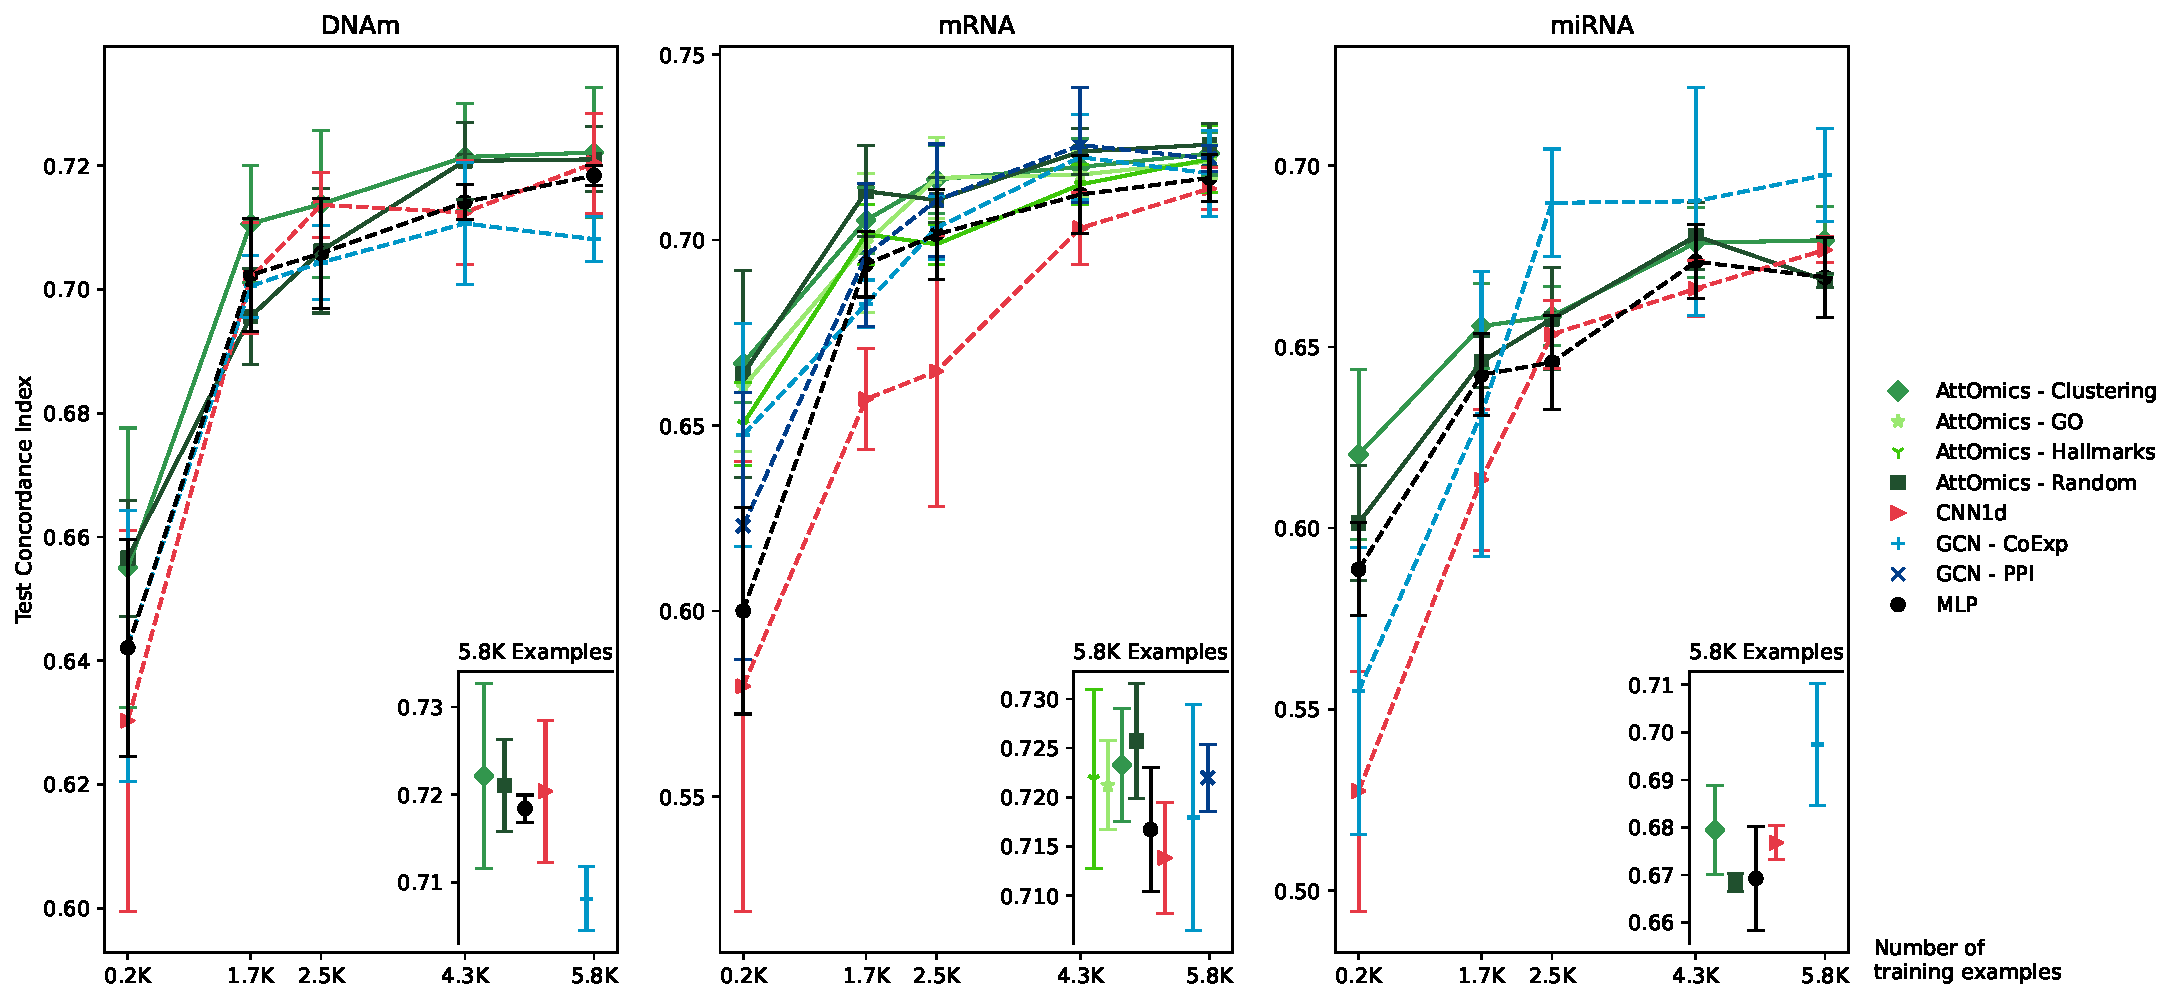
\includegraphics[width=0.9\textwidth]{cancer_type_limited_training_survival.pdf}
	\caption{Concordance Index on the test set according to the size of the training set. }\label{fig:limit_train_cox}
\end{figure}

\begin{table}[htbp]
	\centering
	\caption{Comparison of the time required to obtain predictions from the different models on the test set. }\label{tab:arch_timings}
	\begin{tblr}{
		colspec={
				Q[l,m]
				Q[l,m]
				Q[r,m]
			},%
		row{1} = {guard, c},%
		row{2-Z} = {font=\small},%
		hline{1,Z} = {2pt},%
		hline{2} = {1pt},%
		hline{10,21} = {1pt, dashed},
				cell{2}{1} = {r=8,c=1}{l,m},
				cell{10}{1} = {r=11,c=1}{l,m},
				cell{21}{1} = {r=8,c=1}{l,m},
			}
		Omics & Model                 & Time (s) \\
		DNAm  & AttOmics – Clustering & 0.006    \\
		      & AttOmics – Random     & 0.004    \\
		      & CNN1d                 & 0.078    \\
		      & GNN – CoExp           & 6.280    \\
		      & MLP                   & 0.001    \\
		      & RF                    & 0.046    \\
		      & SVM                   & 5.914    \\
		      & XGBoost               & 0.019    \\
		mRNA  & AttOmics – Clustering & 0.008    \\
		      & AttOmics – GO         & 0.028    \\
		      & AttOmics – Hallmarks  & 0.005    \\
		      & AttOmics – Random     & 0.008    \\
		      & CNN1d                 & 0.178    \\
		      & GNN – CoExp           & 6.623    \\
		      & GNN – PPI             & 2.564    \\
		      & MLP                   & 0.010    \\
		      & RF                    & 0.040    \\
		      & SVM                   & 12.850   \\
		      & XGBoost               & 0.028    \\
		miRNA & AttOmics – Clustering & 0.002    \\
		      & AttOmics – Random     & 0.002    \\
		      & CNN1d                 & 0.006    \\
		      & GNN – CoExp           & 0.326    \\
		      & MLP                   & 0.001    \\
		      & RF                    & 0.270    \\
		      & SVM                   & 20.868   \\
		      & XGBoost               & 0.022    \\
	\end{tblr}
\end{table}

\begin{figure}[htbp]
	\centering
	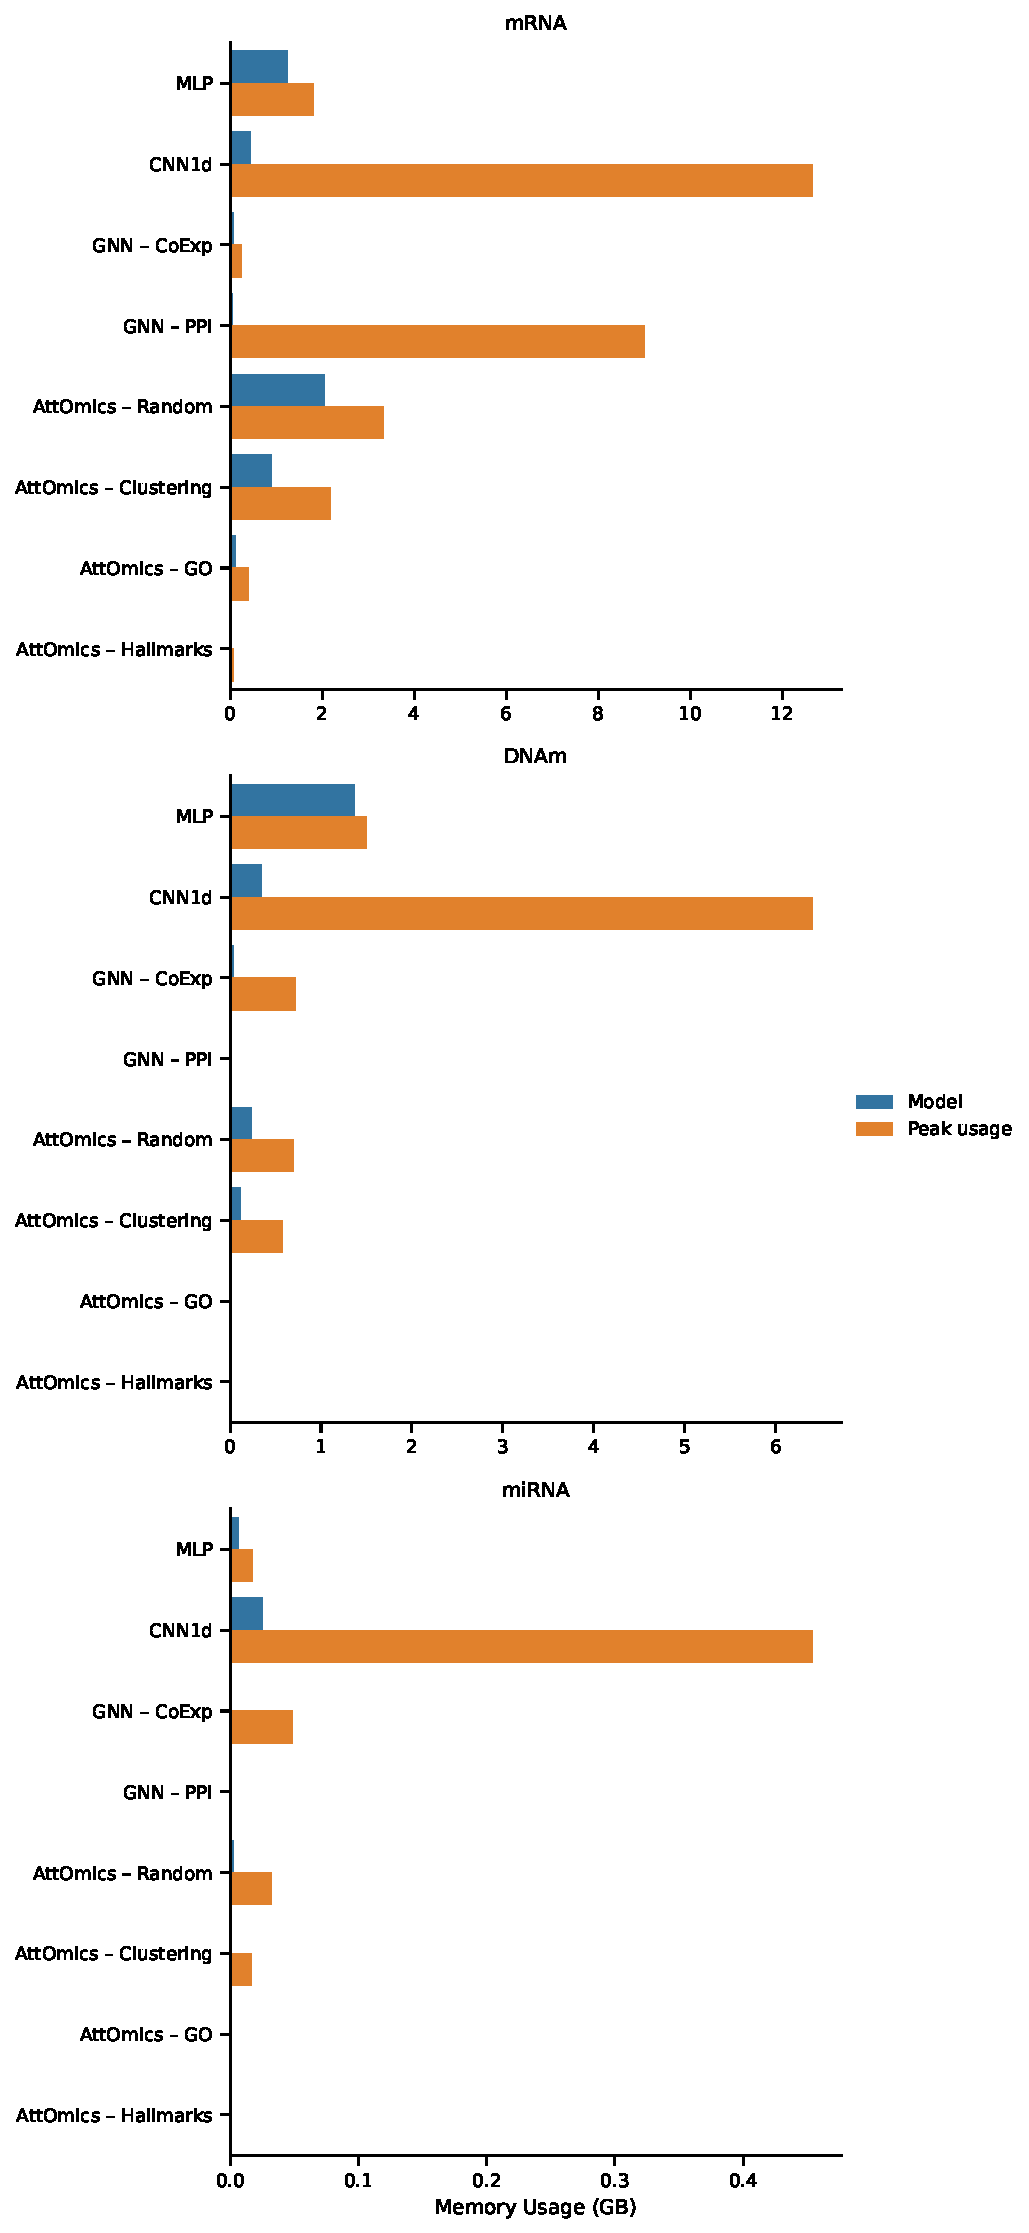
\includegraphics[scale=0.5]{memory_usage_models.pdf}
	\caption{Comparison of the memory usage of the different deep-learning models and the peak of memory usage during inference on the test set.}\label{fig:mem_uasge}
\end{figure}



\begin{figure}[htbp]
	\centering
	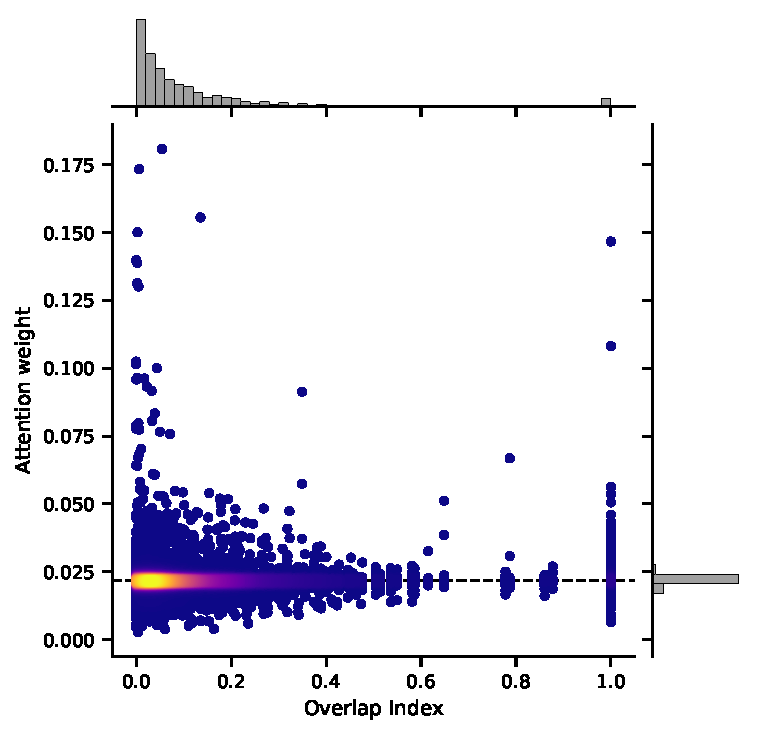
\includegraphics[width=\textwidth]{attention_weight_overlap.pdf}
	\caption{Attention weight and overlap index comparison for grouped based on GO\@. The dashed line correspond to the expected mean attention weight (\(\frac{1}{n_{groups}} \)). Points are colored based on the density of points.}\label{fig:att_w_overlap}
\end{figure}

\begin{landscape}
	\begin{figure}[p]
		\centering
		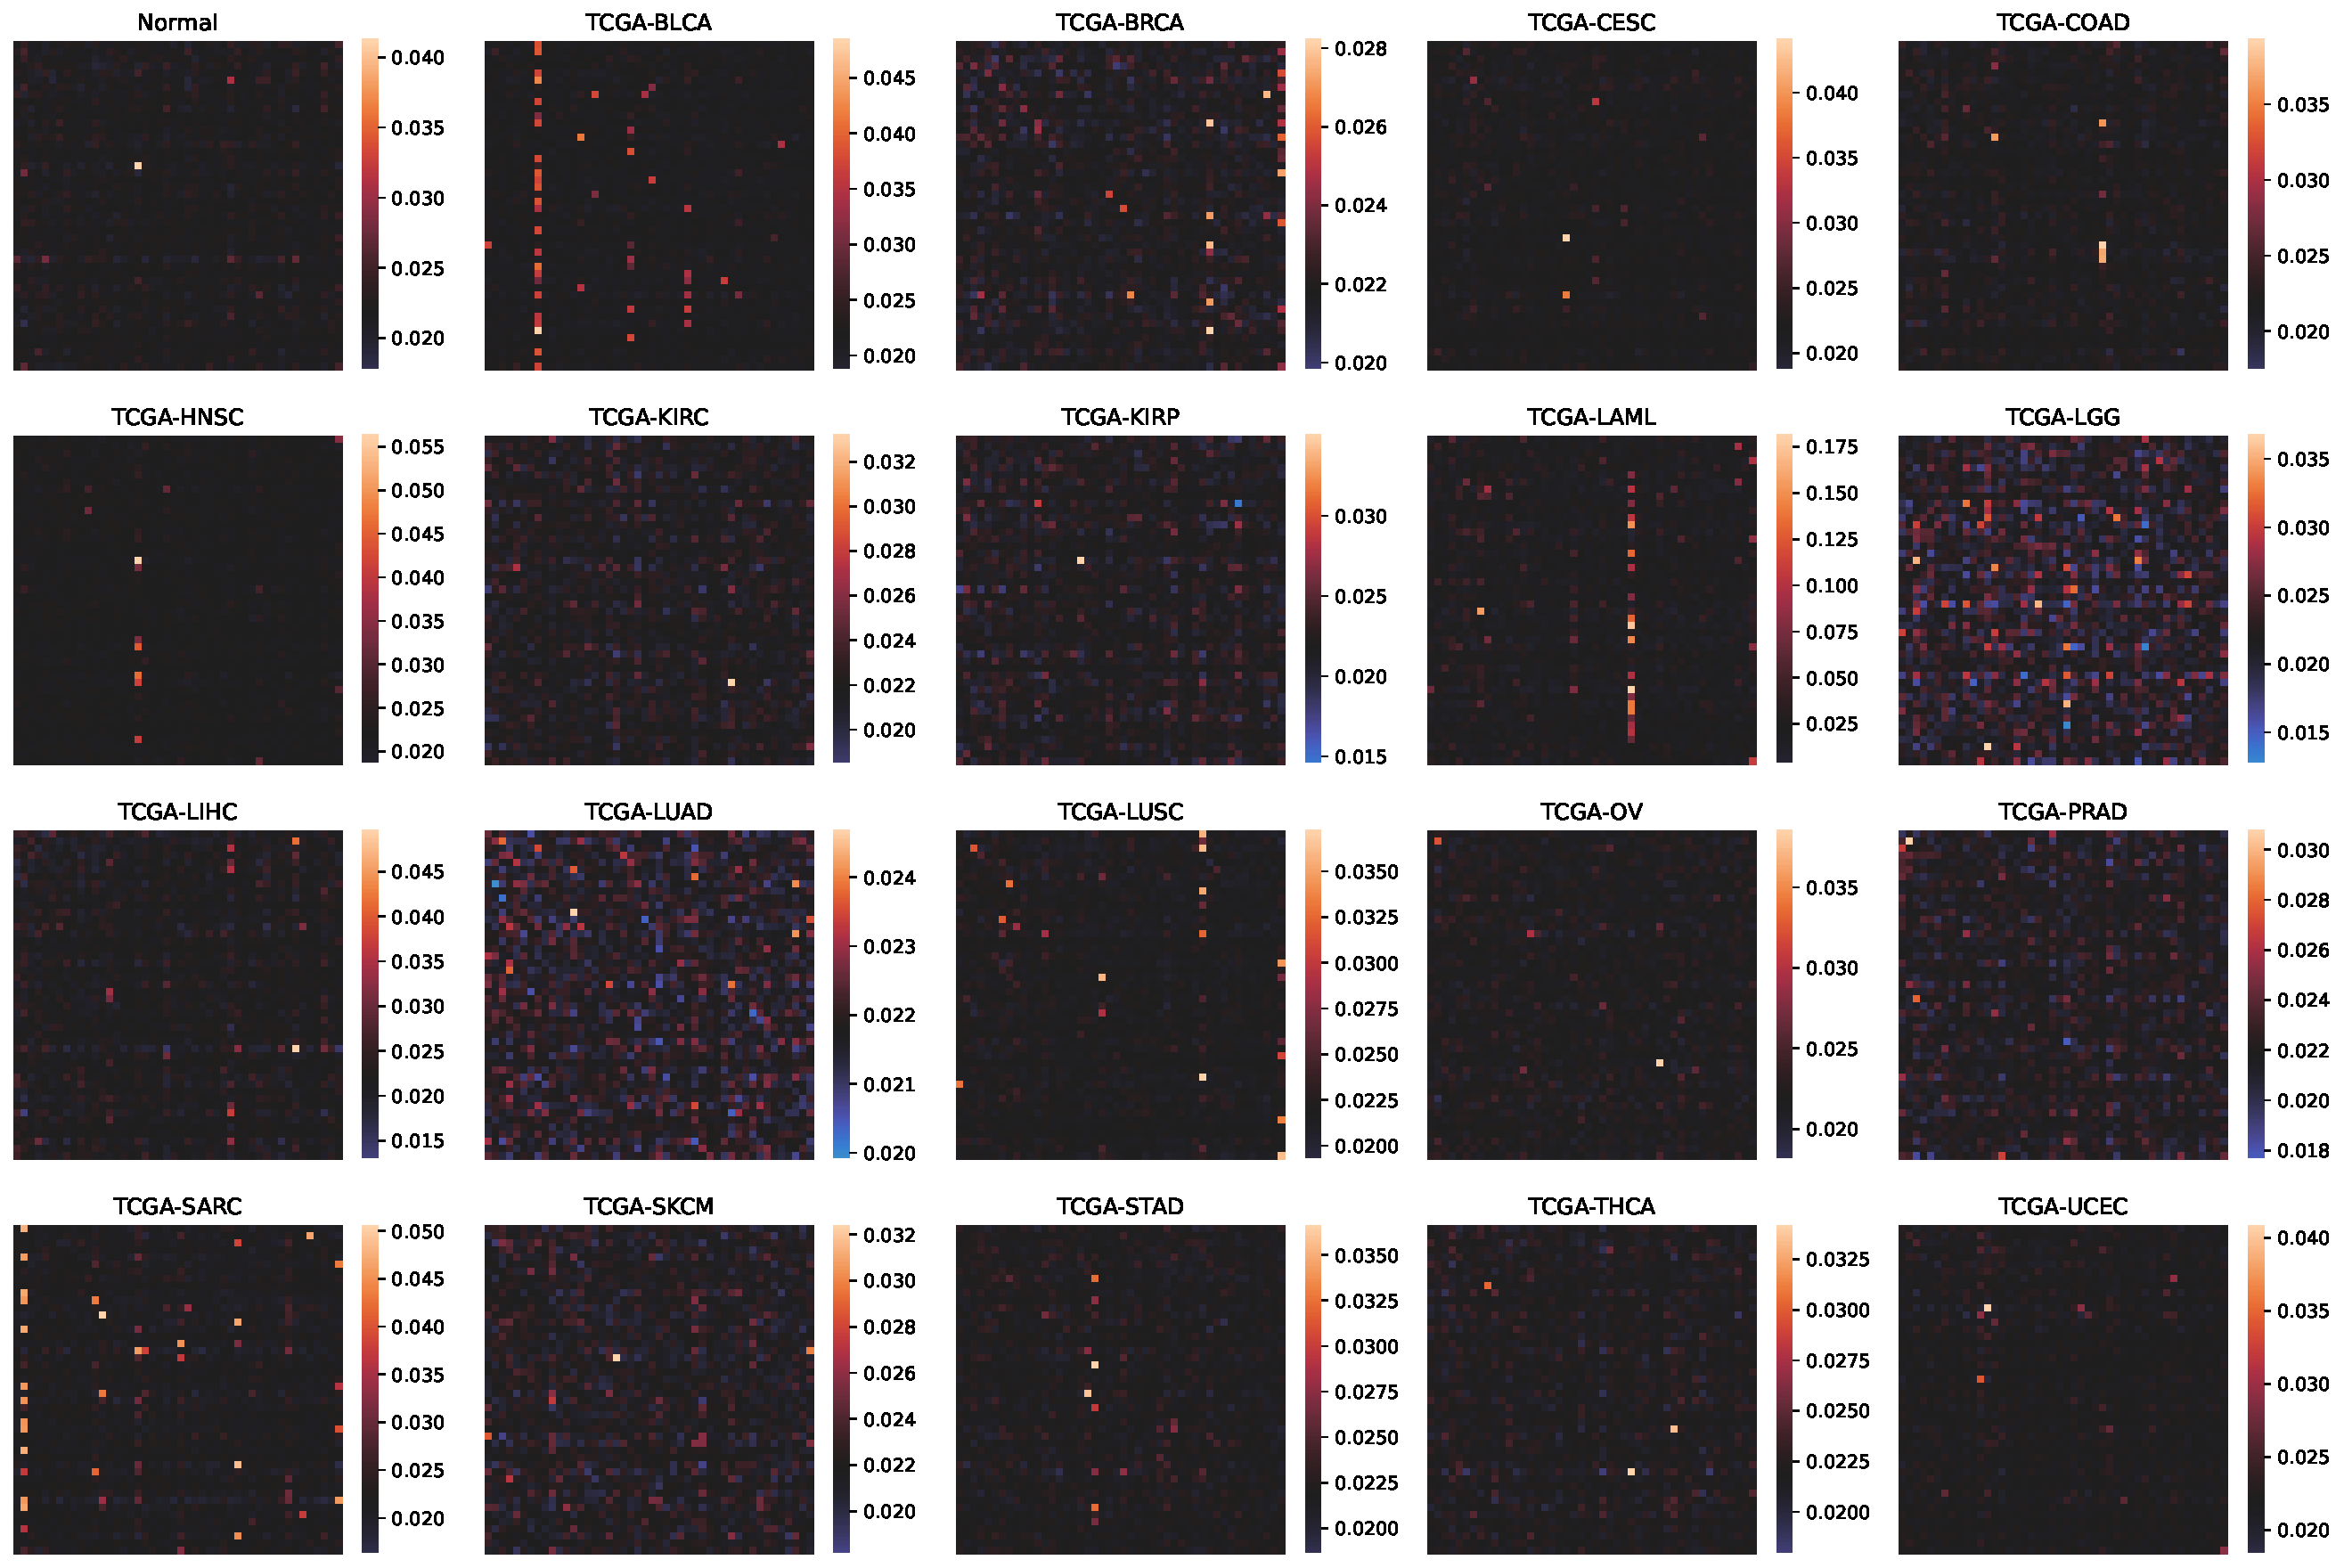
\includegraphics[width=0.9\textheight]{attention_maps_cancer_go_block1.pdf}
		\caption{Attention map visualized per cancer for the first block when grouping with the gene ontology strategy. Attention map per cancer are obtained by taking the mean of the attention map of all patients with the corresponding cancer. }\label{fig:att_map_cancer_go}
	\end{figure}

	\begin{figure}[p]
		\centering
		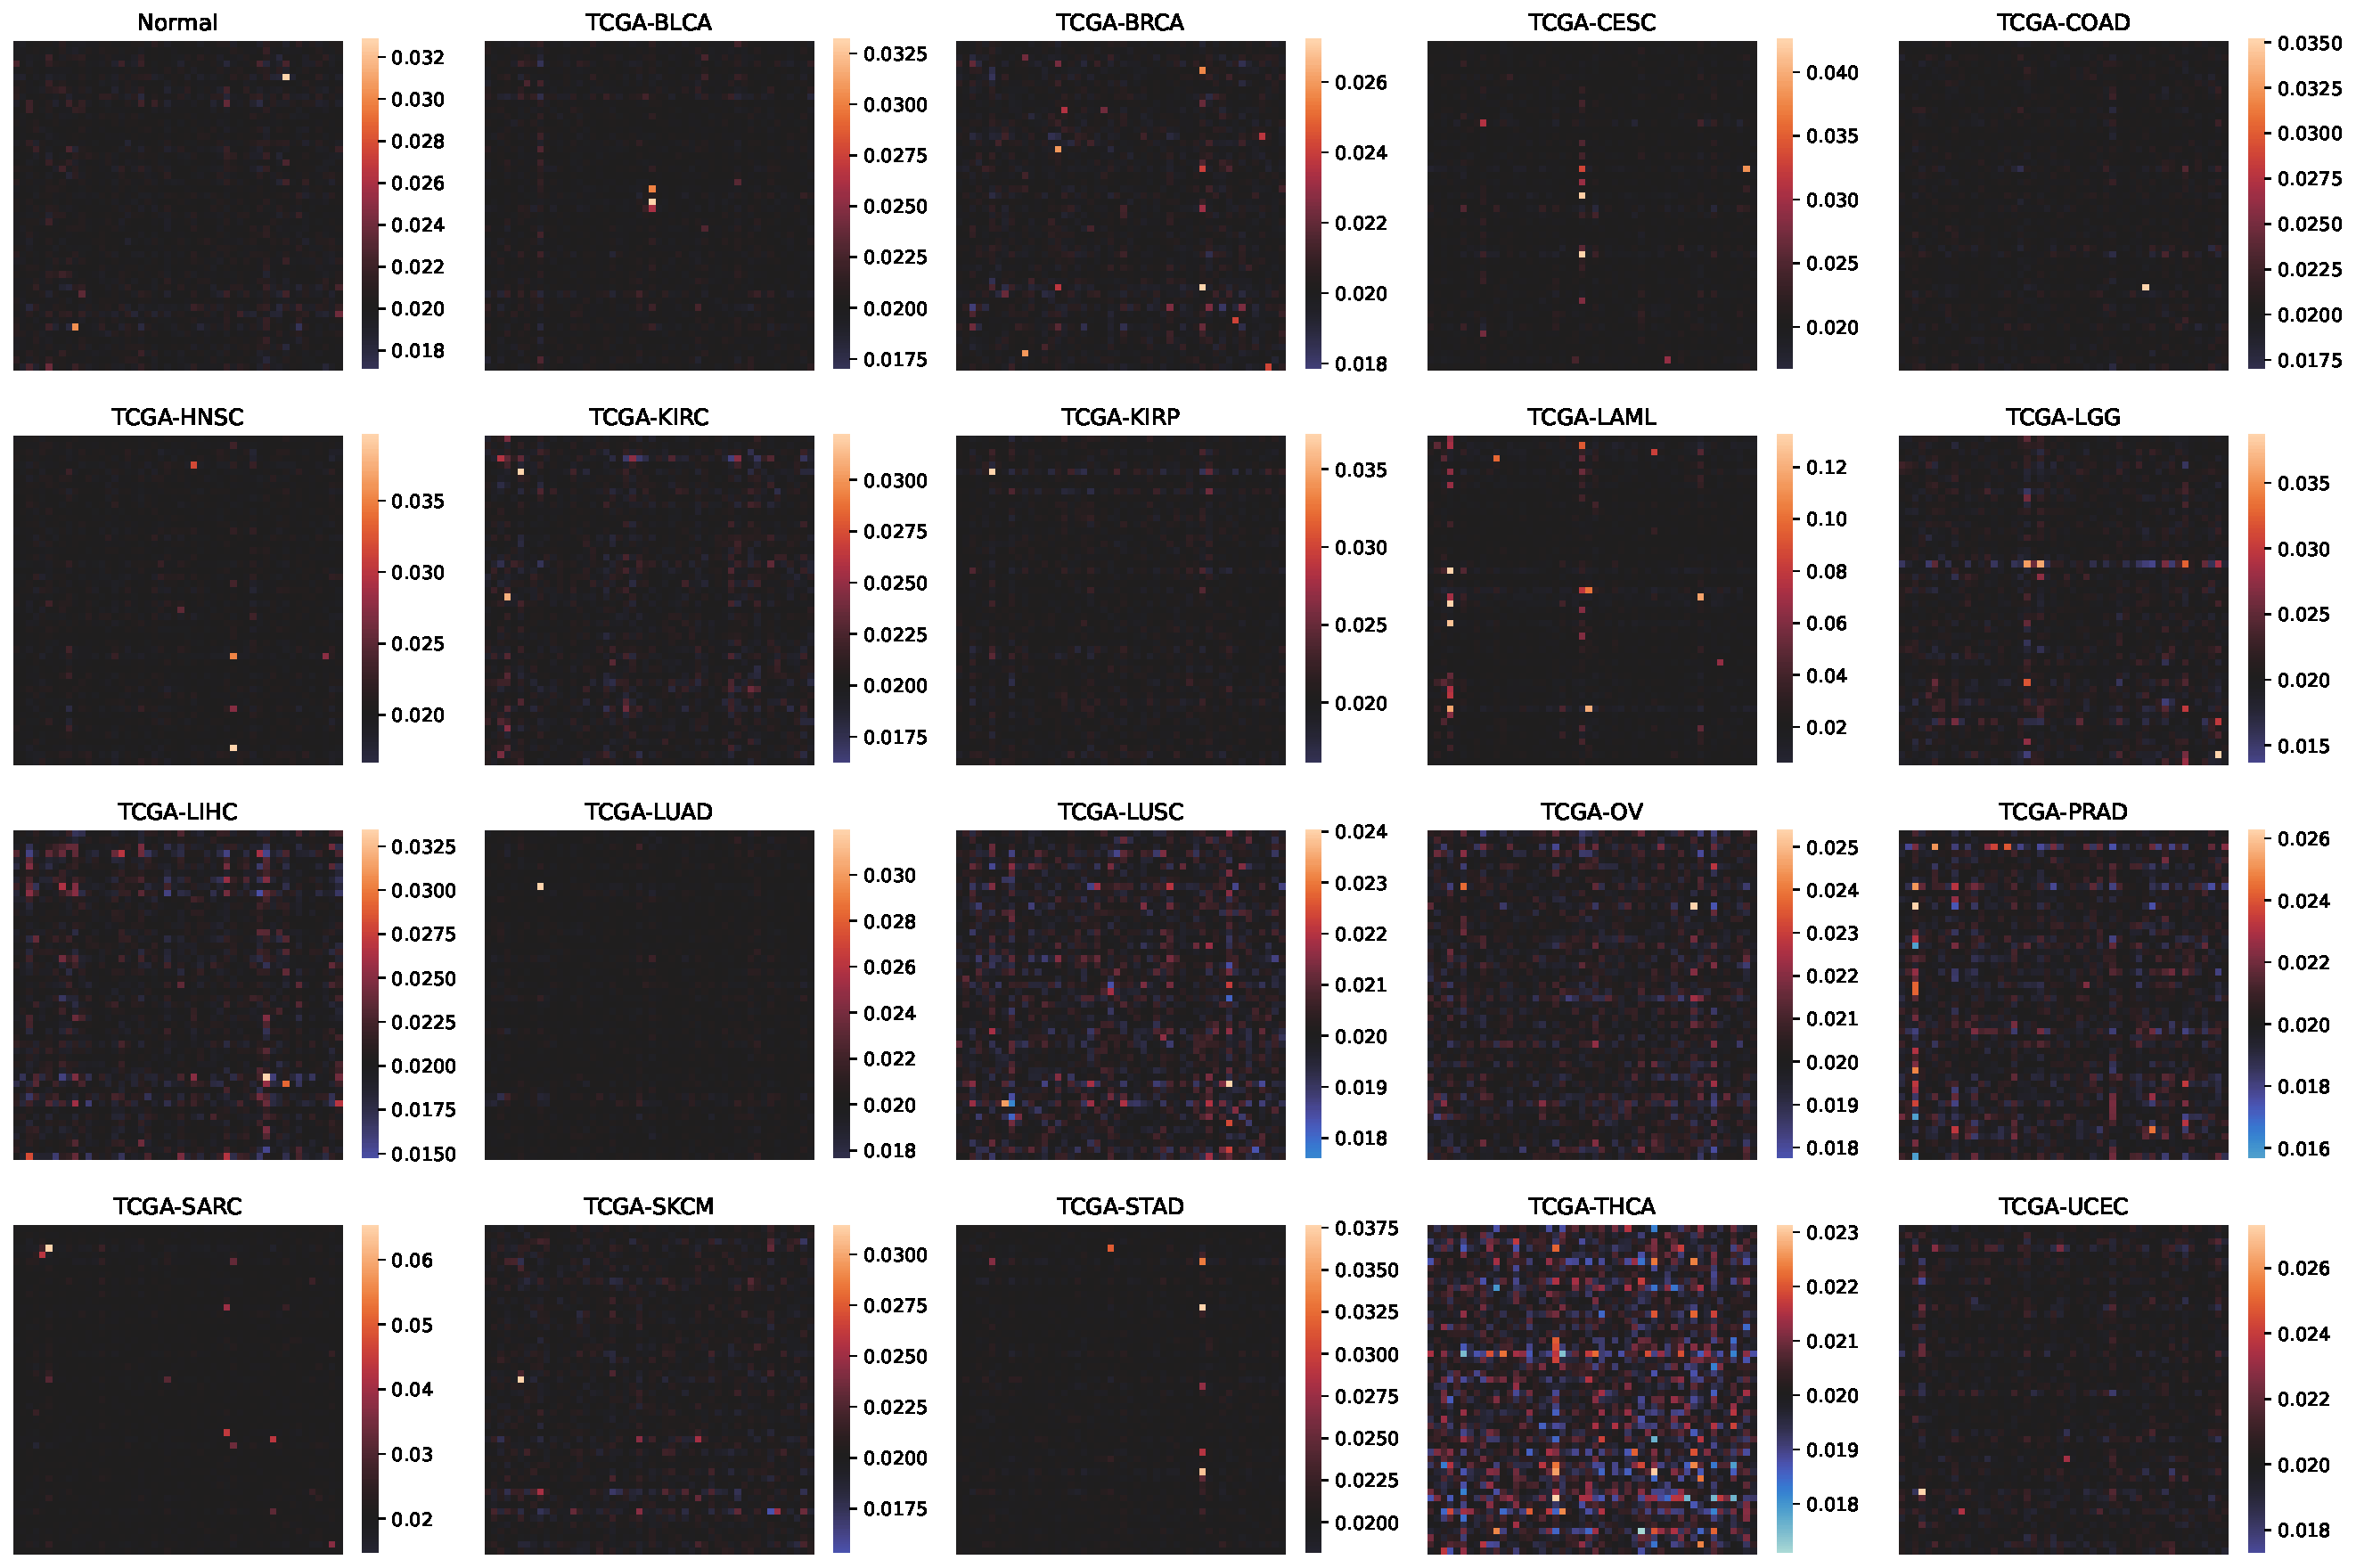
\includegraphics[width=0.9\textheight]{attention_maps_cancer_hallmarks_block1.pdf}
		\caption{Attention map visualized per cancer for the first block when grouping with the hallmarks strategy. Attention map per cancer are obtained by taking the mean of the attention map of all patients with the corresponding cancer. }\label{fig:att_map_cancer_hallmarks}
	\end{figure}

	\begin{figure}[p]
		\centering
		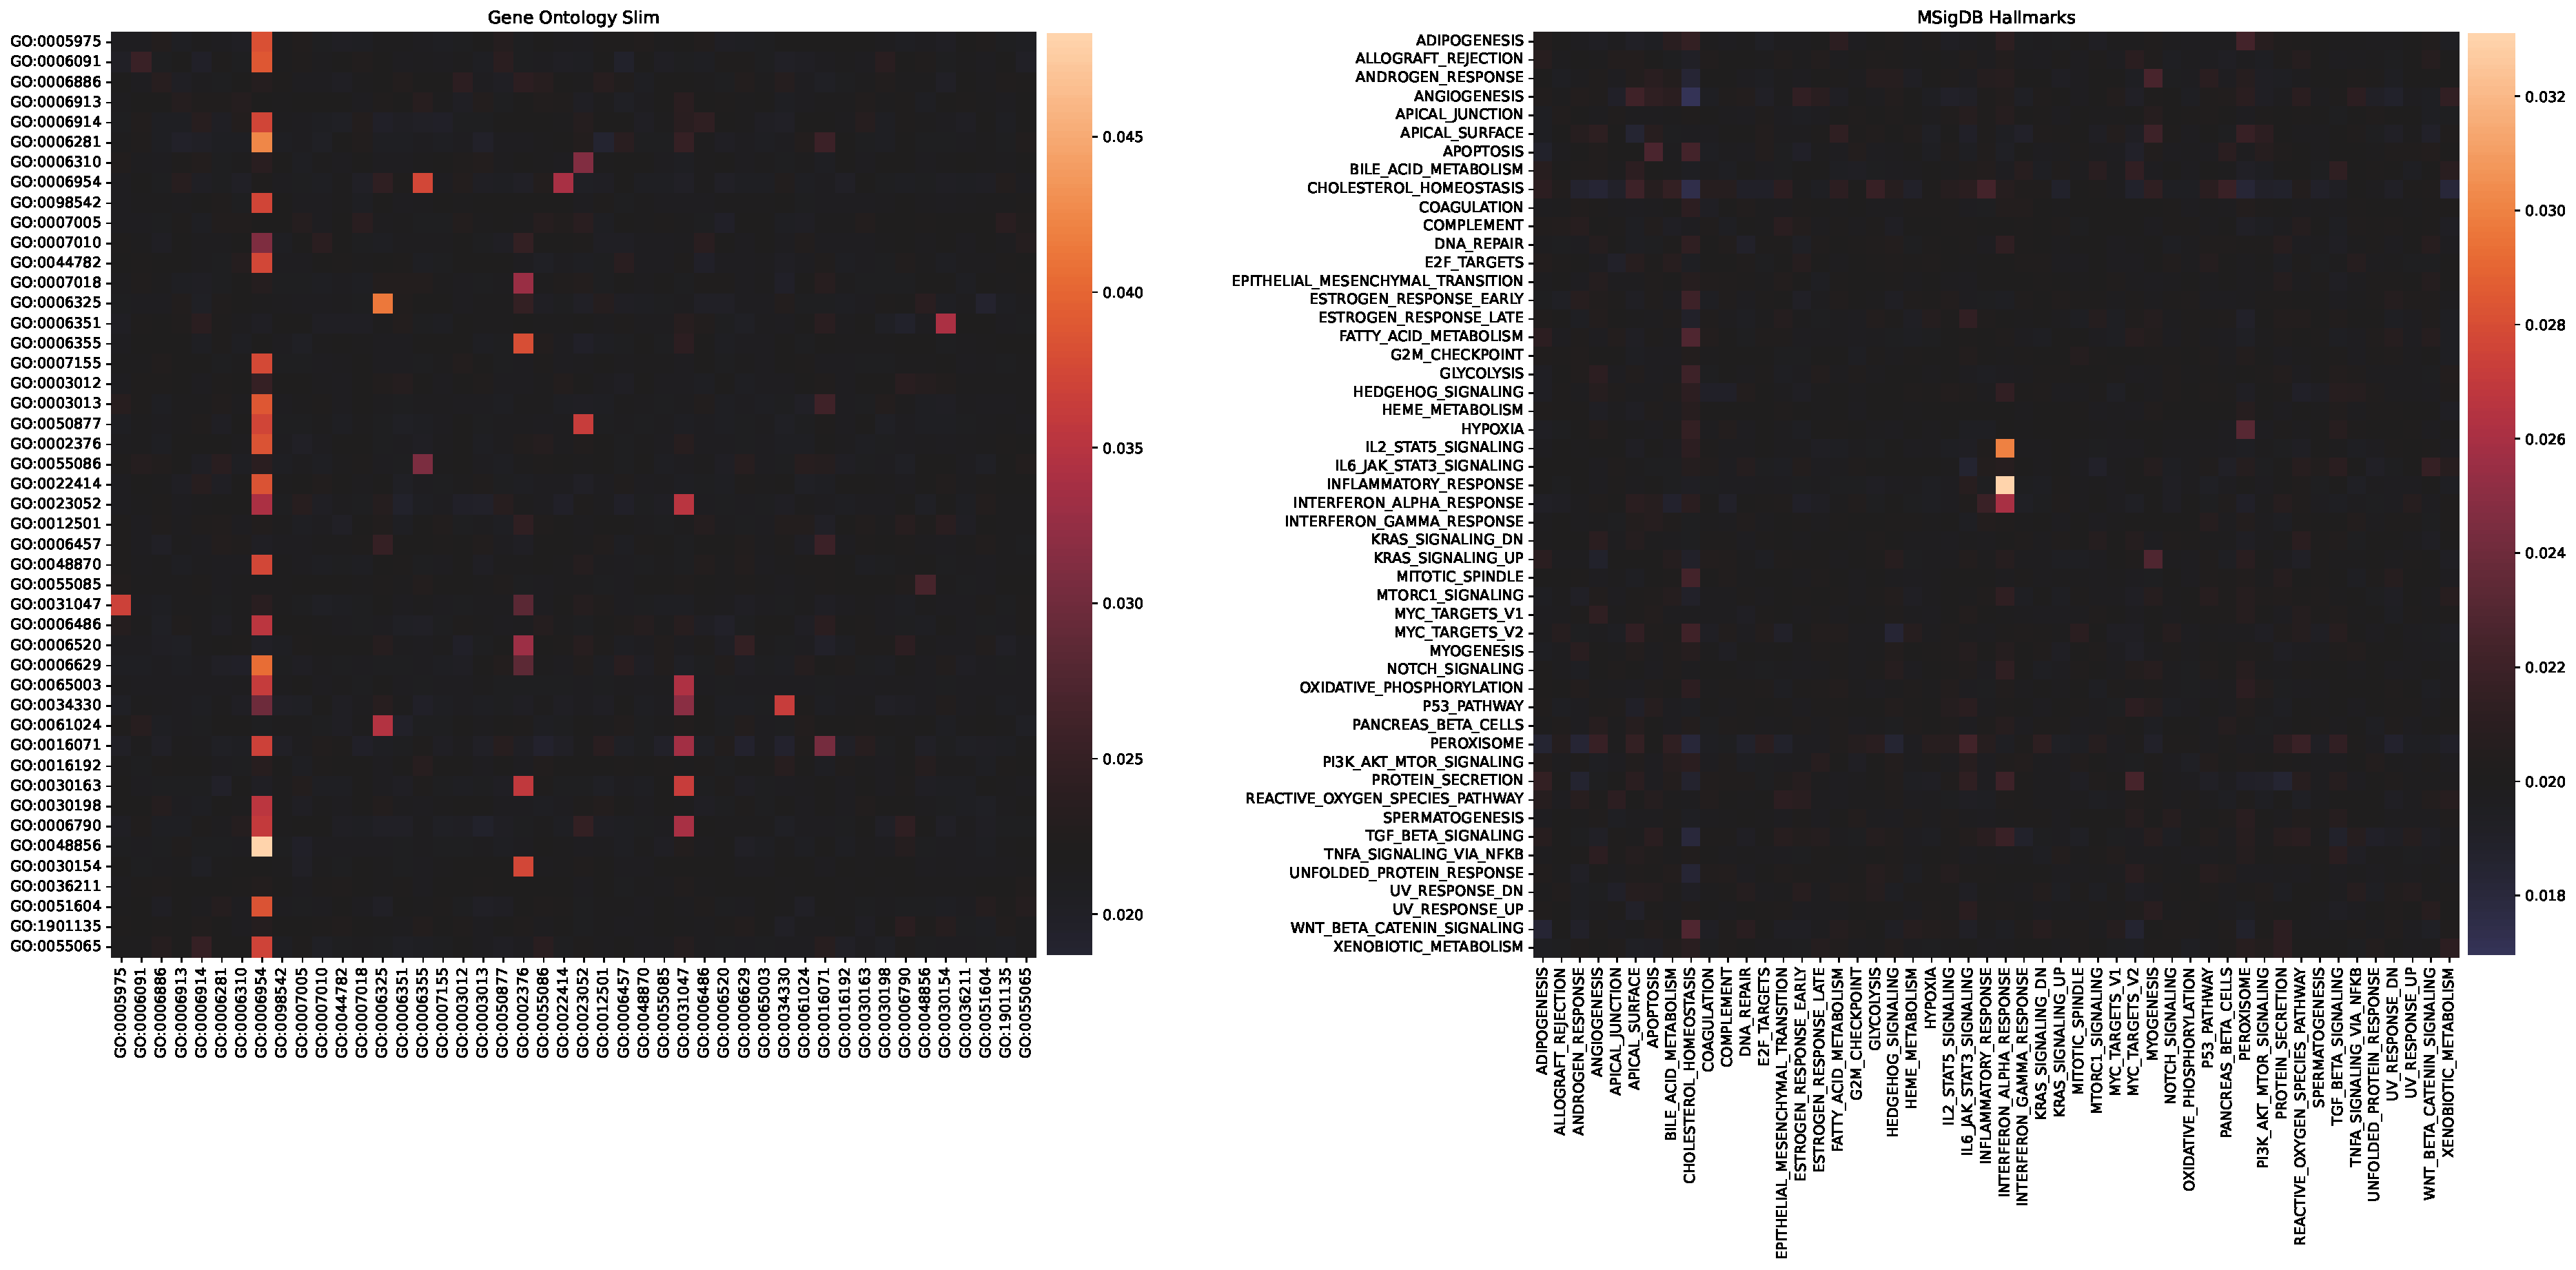
\includegraphics[width=0.9\textheight]{TCGA_BLCA_comparison_attention_go_hallmarks.pdf}
		\caption{Comparison of the attention maps obtained with the gene ontology and the hallmarks grouping strategy. Both attention map highlights interaction involving an inflammatory response group. }\label{fig:att_map_blca_comp}
	\end{figure}
\end{landscape}